\documentclass[letterpaper, 10 pt, journal, twoside]{IEEEtran}
\IEEEoverridecommandlockouts
% \input{archive/main.config.tex}
\usepackage{graphicx}
\usepackage{caption}
\usepackage{subcaption}
\usepackage{soul}
\usepackage[dvipsnames]{xcolor}
\hyphenation{op-tical net-works semi-conduc-tor}
\usepackage{xcolor,listings}
\usepackage{textcomp}
\usepackage{todonotes}
\lstset{upquote=true}
\usepackage{array}
% \usepackage{graphicx}
\usepackage{amsmath}
\usepackage{relsize}
\usepackage{amssymb}
\usepackage{color}
\usepackage{threeparttable}
\usepackage{hyperref}

\usepackage{algorithm}
\usepackage{algpseudocode}
% \usepackage[colorlinks,citecolor=blue]{hyperref}

% \usepackage{draftwatermark}

% Packages for drawing
\usepackage{tikz}
\usetikzlibrary{shapes.geometric, arrows,calc}
\tikzstyle{startstop} = [rectangle, rounded corners, minimum width=3cm, minimum height=1cm,text centered, draw=black, fill=none]
\tikzstyle{io} = [trapezium, trapezium left angle=70, trapezium right angle=110, minimum width=3cm, minimum height=1cm, text centered, draw=black, fill=blue!30]
\tikzstyle{process} = [rectangle, minimum width=3.5cm, minimum height=1cm, text centered, draw=black, fill=orange!0]
\tikzstyle{neuron} = [circle, minimum size=3cm, text centered, draw=black, fill=orange!0]
\tikzstyle{decision} = [diamond, minimum width=3cm, minimum height=1cm, text centered, draw=black, fill=green!30]
\tikzstyle{arrow} = [thick,->,>=stealth]

\usepackage{pgfplots}
\pgfplotsset{compat=newest}
\pgfplotsset{plot coordinates/math parser=false}

\usepackage{booktabs}
\usepackage{multirow}

% \usepackage[maxnames=3,firstinits=true,sorting=none,doi=false,url=true,isbn=false]{biblatex}
\usepackage[maxnames=6,firstinits=true,doi=false,url=true,isbn=false]{biblatex}
\addbibresource{../source/refs.bib}


\def \assumptionSGDfirst {1}
\def \assumptionEWCfirst {2}
\def \assumptionEWCsecond {3}

\pagenumbering{arabic}


%-------------------------------------------------------------------------------

\begin{document}

% ***************************************************
%  TITLE
% ***************************************************
\title{Operational Adaptation of DNN Classifiers using Elastic Weight Consolidation}

\author{Abanoub Ghobrial, Xuan Zheng, Darryl Hond, Hamid Asgari, Kerstin Eder 
\thanks{{\footnotesize
Manuscript  
received ...;
revised ...;  
accepted.... 
Date of publication ...;
date of current version ....

% This research has in part been funded by the ROBOPILOT and CAPRI projects. Both projects are part-funded by the Centre for Connected and Autonomous Vehicles (CCAV), delivered in partnership with Innovate UK under grant numbers 103703 (CAPRI) and 103288 (ROBOPILOT). This research was also supported in part by the UKRI Trustworthy Autonomous Systems Node in Functionality under grant number EP/V026518/1. Also special thanks to S\'everin Lemaignan.

% The Associate Editor for this paper was ....

Abanoub Ghobrial (e-mail: abanoub.ghobrial@bristol.ac.uk), 
Xuan Zheng (e-mail: dq18619@bristol.ac.uk), 
and 
Kerstin Eder (e-mail: kerstin.eder@bristol.ac.uk) 
are with the Trustworthy Systems Lab, Department of Computer Science, University of Bristol, Merchant Ventures Building, Woodland Road, Bristol, BS8 1UB, United Kingdom. 

Darryl Hond (e-mail: darryl.hond@uk.thalesgroup.com),
and
Hamid Asgari (e-mail: hamid.asgari@uk.thalesgroup.com) 
are with Technology and Innovation Research,Thales, Reading, United Kingdom. 

Digital Object Identifier ....
}}}
% \affil{Trustworthy Systems Laboratory, University of Bristol, Bristol, UK}
% \affil{University of West of England, Bristol, UK}
% \affil{Bristol Robotics Laboratory, Bristol, UK}
%
\markboth{IEEE TRANSACTIONS ON INTELLIGENT TRANSPORTATION SYSTEMS VOL. ..., NO. ..., date...}{Ghobrial \MakeLowercase{\textit{et al.}}: Operational Adaptation of DNN Classifiers using Elastic Weight Consolidation}
%
\maketitle

% ***************************************************
%  Abstract
% ***************************************************
\begin{abstract}
\noindent 
Autonomous systems (AS) often use Deep Neural Network (DNN) classifiers to allow them to operate in complex, high dimensional, non-linear, and dynamically changing environments.
%
Due to the complexity of these environments, DNN classifiers may output misclassifications as they experience tasks in their operational environments, that were not identified during development.
%
Removing a system from operation and retraining it to include these new tasks 
% is an expensive process and 
becomes economically infeasible as the number of such ASs increases. 
%
Additionally, such misclassifications may cause financial loss and safety threats to the AS or to other operators in the environment.
%
In this paper, we propose to reduce such threats by investigating how DNN classifiers can adapt their knowledge to learn new information in the AS's operational environment, using only a limited number of observations encountered sequentially during operation. 
%
This allows the AS to adapt to newly encountered information, increasing the AS's classification accuracy and hence its overall reliability. % in its operational environment.
%
However, retraining DNNs on different observations than used in prior training is known to cause catastrophic forgetting or significant model drift. 
%
We investigate how this problem can be controlled by using Elastic Weight Consolidation (EWC) whilst learning from limited new observations. %
%
We carry out experiments using original and noisy versions of the MNIST dataset to represent known and new information to DNN classifiers.
%
Results show that using EWC is effective in controlling the process of adaptation to new information, and thus allows for reliable adaption of ASs to new information in their operational environment.
\end{abstract}

\begin{IEEEkeywords}
Adaptive, Autonomous Systems, Classifier, Elastic Weight Consolidation
\end{IEEEkeywords}
\IEEEpeerreviewmaketitle 


% ***************************************************
%  Main Body
% ***************************************************
\section{Introduction}

Autonomous systems (AS) often are developed using deep neural network (DNN) classifiers to interact and adapt in dynamically changing real-world environments to achieve their intended goals. 
%
The benefit of DNNs driving their usage in autonomous systems is their ability to learn complicated patterns 
% in high-dimensional data 
from complex environments, and thus produce highly non-linear decision boundaries to cope with the complexity of operational environments.
%
However, this also causes ASs to have low trustworthiness as their behaviour is difficult to verify, 
% Generally, trustworthiness increases with increase in reliability\footnote{https://www.vocabulary.com/dictionary/trustworthiness}, 
%
which is often demonstrated through established verification and validation procedures.  
%
A popular example of such ASs, are self-driving cars. Current research shows that for each self-driving car an economically impossible amount of testing is required to verify the system for deployment~\cite{RR-1478-RC}. For which innovative methods of increasing the efficiency of testing and validation are actively being developed to make the process more economically viable e.g.~\cite{chance2020agency,eder2021complete}. 

Generally trustworthiness in autonomous systems is a broad term that tries to quantify trust in relationships, specifically for human-AS interactions~\cite{KateDevitt2018}.
%
The definition of trustworthiness is still maturing and methods for quantifying trustworthiness is still under research.
%
One of the projections of trustworthiness that researchers seem to be settling on is that it constitutes of several properties, examples of these properties are summarised by Wing~\cite{Wing2021}, like \textit{reliability}, \textit{safety}, \textit{security}, \textit{accountability} etc.
%
Reliability, which includes several factors such as accuracy, robustness, and fairness, is off particular interest to the work presented herein. 
%
We are interested in increasing the reliability of ASs by allowing them to perform controlled adaptation to their operational environment, termed \textit{pattern of life} (PoL) tasks.

% On the other hand, t
% The work presented herein aims at increasing the reliability, and hence trustworthiness, of ASs by allowing them to perform controlled adaptation to their operational environment, termed \textit{pattern of life} (PoL) tasks.

% on its operational environment by increasing the performance on its \textit{pattern of life} (PoL) tasks. 
%
PoL is a term used widely in the field of intelligence generation, to refer to intelligence generated by observing and analysing behaviours of any system over a period of time~\cite{Craddock2016}. 
%
We use the term PoL tasks to refer to tasks that an AS encounters during operation. 
%
Specifically, we are interested in PoL tasks that come from a slightly different distribution than used in initially training of the DNN classifiers and thus causes misclassifications.  
%
The method of adapting to PoL tasks complements the verification and validation work on autonomous systems to achieve deployment. 
%
This follows a two-stage approach presented by Koopman~et.al.~\cite{Koopman2020} , which says given that an autonomous system passes some minimum safety validation case, the system is deployed and is improved during operation to increase its reliability over time. 
%
Also allowing the system to adapt to dynamically changing operational environments which may often vary from the expected operational environment at deployment time.

Upon a DNN classifier retraining to learn new information during operation, a reassessment of the safety validation case and testing for verification would be required, which can be impractical to do during operation after every retrain.  
%
How to show the safety compliance of an evolving DNN during operation against a set of requirements or regulations is beyond the scope of this paper, but can be achieved through the use of runtime safety behavioural checkers as was presented by Harper~et.al.~\cite{harper2021safety}. 
%
Also, it can be predicted that a system may exhibit undesirable or unsafe behaviours by assessing how dissimilar the operational input data is to the data used at initial training (before deployment) or at retraining (after deployment during operation) of DNN classifiers as was demonstrated by\textbf{} Hond~et.al.~\cite{Hond2020} and other similar works e.g.~\cite{Schaffer2017, Mandelbaum2017, Xing2019}. 

DNN classifiers uses gradient based optimisation algorithms to learn, which introduces limitations to the adaptation process. 
% which hinders the process of developing reliable adaptive autonomous systems using only encountered observations. These are discussed in the two bullet points below:
%
% This hinders the process of developing reliable adaptive autonomous systems using only encountered observations. 
% These are discussed in the two bullet points below:
% \begin{itemize}
    % \item 
    The gradient optimiser modifies the decision boundary based on the choice of observations used in initial training or retraining. 
    %
    Thus as the observations used in retraining the classifier change between different operational environments, the decision boundary will adapt accordingly, which may result in the reliability of the DNN classifier changing as the system alternates between operational environments. 
    %
    This can be tackled through the usage of PoL adapted classifiers, motivated by our work, tagged to each operational environment of the system and decoupled from each other. 
    
    % \item 
    Additionally, when a DNN classifier encounters a situation, which results in a misclassification, there is a few observations that can be as little as a single observation to use for retraining (adaptation). 
    %
    Retraining using the available new observations results in significant \textit{model drift}\footnote{Model drift or forgetting can be defined as some major or minor decrease in the performance of a DNN on a set of tasks. Catastrophic forgetting, on the other hand, is a drastic decrease in the performance of all learnt tasks.} or in a phenomenon known as \textit{catastrophic forgetting}~\cite{Goodfellow2014}. 
    %
    To generally avoid that, the new observations are added to the original dataset used in initial training and the classifier is fully retrained. 
    %
    Full retraining, however, can be very cumbersome to do during operation. 
    %
    Alternatively, the \textit{learning rate}\footnote{The learning rate hyper-parameter controls the rate at which the model's weights are modified during training.
    % The hyper-parameter used in controlling how much the neural network model is flexible to drift. 
    The lower the learning rate the less drift.} 
    can be set to be very low in order to avoid the model from drifting. 
    %
    This unfortunately causes the DNN model not to learn information sufficiently from new observations because the learning rate is low, restricting the model from drifting to adapt to new information. 
    %
    Trying to optimise the learning rate still results in significant if not catastrophic forgetting, as shown later by the results. 
    %
    This raises the need for a method to protect features of the DNN classifier important for preserving performance on old information, whilst still providing flexibility for the model to drift and adapt to PoL tasks.
    %
    There are several methods in the literature that have been demonstrated to be able to protect previous information in DNNs,.e.g. elastic weight consolidation (EWC)~\cite{Kirkpatrick2017} is one of the very successful methods at doing so and is the method we have adopted in this paper. 
    %
    Further information on the rationale behind choosing EWC is provided in later sections of the paper.
    
% \end{itemize}

This paper aims at discussing the following two research questions:

\textbf{Research question 1 (RQ1):} Can the use of EWC allow for DNN classifiers to benefit from learning new encountered observations whilst controlling the forgetting of previous knowledge?
% Can the use of EWC allow for higher learning rates to be used during retraining to allow for both i) the DNN classifier to improve its benefit from learning new encountered observations and ii) whilst controlling the forgetting or model drift on previous knowledge? 

\textbf{Research question 2 (RQ2):} Does learning from a limited number of relevant observations generalises the classifier’s performance to the new tasks?
%Based on a positive outcome of research question 1, can this be used to allow for pattern of life adaptation of autonomous systems?

% We develop a retraining pipeline using EWC and evaluate its performance against the use of SGD alone.

The process of continual learning or adaptation of an autonomous system also involves the detection of incorrect behaviours and supply of correct labels for the new observations encountered and used in retraining. 
%
This can be achieved through the use of oracles~\cite{Barr2015,Zhang2020} to provide a ground truth reference and we aim to investigate this further in upcoming works, but in this paper we assume that the correct labels are available for misclassified observations.

% \subsection{Contribution and structure of the paper}
In this paper, we develop a retraining pipeline for PoL adapting DNN classifiers. 
% that can be used for the adaptation of DNN environment specific pattern of life DNNs during operation of an autonomous system.
%
A shortcoming of many of the experimentation reported in the literature is that it is always assumes that sufficient data is available for learning new information. 
%
This is not true with real time systems that may have as little as one observation to retrain on. We do not make this assumption in our experimentation and retrain on limited instances of new information.

We control the forgetting of older information by using EWC which is shown to be one of the most promising techniques for overcoming catastrophic forgetting based on Parisi~et.al.~\cite{Parisi2019}.
% EWC learns using a Bayesian framework, making it very suitable for the application of PoL learning. 
% 
The retraining pipeline learns in a fashion that tries to balance between the original tasks and the PoL tasks encountered during operation based on some chosen criteria. 
% This pipeline can be used to modify DNNs for regional PoL tasks for autonomous systems.

In the next section, we introduce some preliminaries that will help in understanding the rationale behind the way the retraining pipeline was created. 
%
Section~\ref{sec:method} introduces the methodology, which includes the challenges, the pipeline, and the rationale behind it.
%
Experimentation is presented in Section~\ref{sec:experimentation}, along with the results and discussion. 
%
We conclude and discuss future works in section \ref{sec:conclusions}.


\section{Related work}

The problem of forgetting when retraining is a well-known issue with DNNs, which prevents the application of continual learning in autonomous systems.
%
Over the past decade, there has been an increase in focus by researchers on the topic of forgetting in DNNs. 
% during continual learning, which is due to the limitation of full retraining.
%
In continual learning, full retraining is usually resorted to as it gives the most guarantee that no previous information will be lost, where new observations are simply added to the original dataset and the neural network is trained from scratch e.g. \cite{Stocco2021}. 
%
Whilst this might be the easiest approach, it is limited to certain types of systems and is not sustainable for dynamic autonomous systems where training on the original tasks takes hours or days to complete.
%
The increase in interest on the topic of forgetting has also been encouraged by published research investigating the limitations of continual learning in gradient optimised DNNs, e.g.~Goodfellow~et.al.~\cite{Goodfellow2014}, where they studied the effect of the relationship between different learnt tasks and catastrophic forgetting for different optimisation algorithms in the literature. 

In order to solve these limitations of continual learning, researchers have explored numerous techniques that try to conserve or protect previously learnt information when learning incrementally instead of full retraining.
%
Conserving learnt information can be achieved by freezing weights e.g.~\cite{Wang2017,Li2018c}, or introducing penalisation terms that 
restrain weights of importance to old information in the DNN from significantly changing. 
% Therfore avoiding the model does not drift significantly and hence minimises forgetting.
% from being lost not forgetting previous infomration.
% give less flexibility to weights of 
% importance to  
% less importance to previously learnt information, whilst restraining weights important for previously learnt information from deviating. 
%
Thus optimising the performance of a DNN between both the previous and new learnt information e.g.~\cite{Kirkpatrick2017,Zenke2017,Maltoni2019a}.

Inspired from Dopaminergic neurons in mammalian brains which allows for rapid and isolated adaptation in the synapses of neurons, Allred et.al.~\cite{Allred2020} tried to solve the problem of catastrophic interference in Spiking Neural Networks (SNNs).
%
They introduced an artificial dopaminergic neuron in each layer of the spiking neural networks. The role of which is to control neurons that are allowed to adapt during retraining. 
%
If a neuron output is above a certain threshold for previously learnt information, then it is deemed as important for old tasks and should not be altered, thus the artificial dopaminergic neuron stops it from changing during retraining on new information, whilst allowing neurons of less or no importance to previous tasks to be altered.
%
By measuring the firing threshold in neurons they also detect when novel data is experienced.

Elastic weight consolidation (EWC), ~\cite{Kirkpatrick2017}, is another approach for continual learning developed for DNNs that has shown very promising results in the literature.
%
EWC uses a Bayesian framework to learn continuously, whereby the old information learnt is approximated in a term and included in the loss function used in retraining.  
%
% Such that 
This results in weights that have more influence on the classification of old information to 
% that have more significance on the decision-making of old information 
have less flexibility to deviate.  Therefore, as new information is learnt the EWC framework allows the previously trained model to drift in a direction that allows it to optimise for both old and new information simultaneously.   

These approaches discussed above are examples that fall under the category of regulatory techniques in continual learning, mainly focusing on modifying existing neural network resources to learn new information whilst minimising forgetting.
%
A comprehensive and thorough review is provided by Parisi~et.al.~\cite{Parisi2019}, where they cover other continual learning categories such as architectural techniques, whereby existing neurons trained on previous information freeze and new neurons are added to learn new information.
%
They also cover rehearsal and memory replay approaches which cover methods that try to mitigate the problem of forgetting by retraining the system occasionally on subsets of previously learnt observation to avoid the model from completely drifting from previously learnt information. 

Kemker~et.al.~\cite{Kemker2018a} introduced their own metrics to compare between different developed schemes that avoid catastrophic forgetting.
%
Based on their experimentation they reach the conclusion that the achieved optimal performance for each of the developed schemes varies depending on the incremental training paradigm and type of data used. 
%
They also conclude based on their results that all the techniques investigated demonstrate that the challenge of catastrophic forgetting is not yet solved.
%
This demonstrates that there is no one-size-fits-all solution that can generalise to all dynamically changing environments of an autonomous system.  
%
Therefore a solution ought to be developed specifically for each of the changing environments of an autonomous system, which is similar to how the human brain adapts to learn thoroughly tasks and rare instances in its operational environments or pattern of life. 

\section{Preliminaries}\label{sec:preliminaries}
In this section we outline definitions for key terms that is used in subsequent sections.
%
To also gain an understanding of the requirements and limitations of 1) gradient optimisation algorithms, specifically the stochastic gradient decent (SGD) algorithm and 2) EWC, we go through their derivations in this section and note down any assumptions that the SGD or EWC were based on, to ensure they are satisfied in the developed methodology. 

\subsection{Definitions} \label{definitions}
\subsubsection{Observation}
An observation is a data point. 

\subsubsection{Instance}
An instance refers to several observations of the same task captured within a time window in a video feed of the AS.
%
A \textit{new instance} is a misclassified instance.

\subsubsection{Training and testing datasets}
The set of observations used in training the DNN are referred to as the training dataset.
%
These observations are random samples from the distribution representing the (expected) operational environment of the system.
%
Equivalently, a test dataset refers to other random samples from the same distribution used to verify how well the trained network has generalised to the whole distribution.
%
Training and testing datasets have \textit{labels} associated with them, which provides a reference to the correct classification during constructing or verifying the DNN.

\subsubsection{Classes}
Represents the possible output classifications of a DNN, which forms the output layer.
%
A new class represents a \textit{new classification}. 
%
Therefore, if a new classification is to be added to a DNN, an architectural change will be required to the output layer of the DNN.

\subsubsection{Task}
The word \textit{task} is used very subjectively in the continual learning literature, depending on the context of the research. 
%
We try to capture the different definitions of a task in the curly brackets below, by explaining what a new task is considered to be, and highlight in bold the definition we adopt in this paper.
%
\begin{equation*}
  \text{A new \textit{task} can be a~} 
    \begin{cases}
    %   \text{pattern of a novel class}\\
     \text{novel class}\\
      \text{novel pattern of all classes}\\
      \text{novel pattern of a single class}\\
      \text{novel noise applied to all classes}\\
      \text{\textbf{novel noise applied to a single class}}
    \end{cases}       
\end{equation*}

For example, if a neural network's task was to classify numbers from 0 - 9 in English, then a new task (novel class), would be digit 10.
%
A new task (novel pattern of all classes), can be the set of digits from 0 - 9 in a different language. Thus, the same labels of zero to nine but the pattern that represents the number has changed.
%
Equivalently, novel pattern of a single class, is a task that represents only one digit following a new pattern instead of all the digits.  
%
On the other hand, a new task (novel noise applied to all classes), for example, can be Gaussian noise applied to all of the digits from 0 - 9 in English; or a new task (novel noise applied to a single class) can be Gaussian noise applied to only a single digit from 0 - 9.  In this paper we adopt the latter definition unless otherwise stated.  

% \subsubsection{Oversampling}
% Inspired by Synthetic Minority Oversampling Technique (SMOTE)~\cite{Chawla2002}\cite{Stocco2021},  the term \textit{oversampling} is used here to refer to creating more samples from an observation

% instance, whether generated using synthetic techniques or through capturing samples from a video feed to create more observations to represent a new task, this is not to be confused with the generic definition of oversampling in signal processing, that refers to sampling a signal at a sampling frequency higher than the Nyquist frequency~\cite{Byrne2020}. 


\subsection{Stochastic Gradient Descent (SGD)}\label{sec:gradient_decent}
Figure~\ref{fig:neuron_connected} shows the computation in a single artificial neuron of a DNN.
%
Where $[x_1, ..., x_K]$ and $[w_1,... ,w_K]$ are the set of inputs and weights into the neuron respectively. The term $b$ is the bias and $x_{out}$ is the output of the neuron as shown by Equation~\ref{neruon_equation}.
ReLU is the popular rectified linear unit activation function used in DNNs given by Equation~\ref{Relu}, refer to ~\cite{Huang2020b} for a more thorough formal representation of DNNs with several neurons and layers. 

\begin{figure}[h!]
    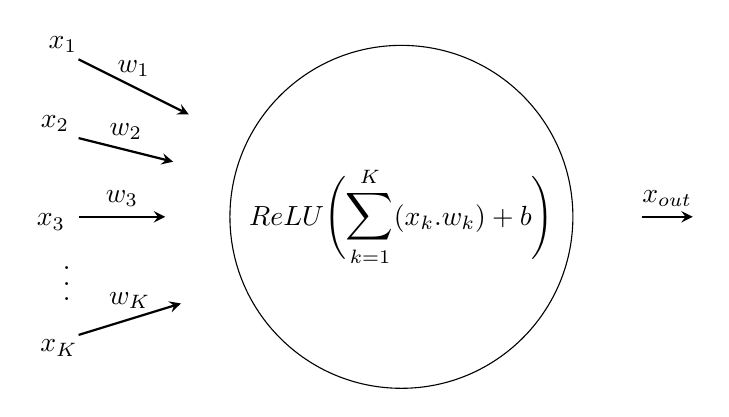
\begin{tikzpicture}[node distance=3.5cm]
 
        % \node (neuron1) [neuron, fill=none, minimum size=2cm, xshift=3.8cm] {$ReLU \Bigg( \mathlarger{\mathlarger{\sum}}_{k=0}^{K} (x_{k,z-1}.w_{x_k,z-1})+b_{k,z})\Bigg)$};
        
        \node (neuron1) [neuron, fill=none, minimum size=2cm, xshift=3.8cm] {$ReLU \Bigg( \mathlarger{\mathlarger{\sum}}_{k=1}^{K} (x_{k}.w_{k})+b\Bigg)$};
        
        %  \node (activation) [process, draw=white, minimum width=4cm, minimum height=2cm, text width=8cm, text height=5cm, text depth = 0 cm, yshift=0cm, xshift=0cm, align=left] {$ReLU(x_{k,z})$};
         
        %  \node (activation) [process, fill=none, minimum width=2cm, minimum height=1cm, yshift=0cm, xshift=7cm, align=center] {{$ReLU(x_{k,z})$}};
    
    
         \draw[arrow] (-0.3,2) -- node[anchor=south, xshift=-0.9cm, yshift =0.3cm] {$x_{1}$} node[anchor=south, yshift =0cm] {$w_{1}$} (1.1,1.3);
         
         \draw[arrow] (-0.3,1) -- node[anchor=south, xshift=-0.9cm, yshift =0.1cm] {$x_{2}$} node[anchor=south, yshift =0cm] {$w_{2}$} (0.9,0.7);
         
         \draw[arrow] (-0.3,0) -- node[anchor=south, xshift=-0.9cm, yshift =-0.3cm] {$x_{3}$} node[anchor=south, yshift =0cm] {$w_{3}$} (0.8,0);
         
         \draw[arrow] (-0.3,-1.5) -- node[anchor=south, xshift=-0.9cm, yshift =-0.6cm] {$x_{K}$} node[anchor=south, yshift =0cm] {$w_{K}$} node[anchor=south,xshift=-0.8cm,yshift =0.5cm] {$.$} node[anchor=south,xshift=-0.8cm,yshift =0.3cm] {$.$} node[anchor=south,xshift=-0.8cm,yshift =0.1cm] {$.$}  (1,-1.1);
         
        % \draw[arrow] (0,1.5) -- node[anchor=south, xshift=-1.3cm, yshift =0.3cm] {$x_{1,}$} node[anchor=south, yshift =0cm] {$w_1$} (2.2,0.6);
         
        %  \draw[arrow] (0,0.75) -- node[anchor=south, xshift=-1.3cm, yshift =0.1cm] {$x_2$} node[anchor=south, yshift =0cm] {$w_2$} (2.1,0.3);
         
        %  \draw[arrow] (0,0) -- node[anchor=south, xshift=-1.3cm, yshift =-0.3cm] {$x_3$} node[anchor=south, yshift =0cm] {$w_3$} (2.05,0); 
        
        %  \draw[arrow] (0,-1.5) -- node[anchor=south, xshift=-1.2cm, yshift =-0.9cm] {$x_K$} node[anchor=south, yshift =0cm] {$w_K$} node[anchor=south,xshift=-1.2cm,yshift =0.3cm] {$.$} node[anchor=south,xshift=-1.2cm,yshift =0.1cm] {$.$} node[anchor=south,xshift=-1.2cm,yshift =-0.1cm] {$.$} %(2.25,-0.6);
        
         
        \draw[arrow] (6.85,0) -- node[anchor=south] {$x_{out}$} (7.5,0);
        
    \end{tikzpicture}
\caption{Artificial neuron in a DNN}
\label{fig:neuron_connected}
\end{figure}


\begin{equation} 
 x_{out} = ReLU \Bigg(\mathlarger{\mathlarger{\sum}}_{k=0}^{K} (x_{k}.w_{k})+b \Bigg)
 \label{neruon_equation}
\end{equation}
\begin{equation} 
    ReLU(x) = 
        \begin{cases}
          x, & \text{if}\ x\geq0 \\
          0, & \text{otherwise}
        \end{cases}
\label{Relu}
\end{equation}

%


\textit{Training} a DNN refers to tweaking the values of the weights and the biases for each neuron in a DNN so that it achieves the desired outputs for the provided observations (training dataset). 
%
This is achieved by minimising a \textit{loss function}, $\mathcal{L}$, that compares between the DNNs predicted output $\hat{y}$ (for a neural network comprising of one neuron $\hat{y} = x_{out}$) and the target output $y$ i.e. the label. 
%
A method for doing this comparison is by using the mean squared error given by Equation~\ref{eq:mean_square_loss}, where $N$ is the number of observations used in training.
\begin{equation}
    \mathcal{L} = \frac{1}{N} \mathlarger{\mathlarger{\sum}}_{i=1}^{N} (y_i-\hat{y}_i)^2
    \label{eq:mean_square_loss}
\end{equation}

The aim during training is to minimise the difference between the predicted outputs of the DNN and the target output, which means to identify where a local minimum is i.e. gradient is zero. 
%
This is achieved numerically using gradient-based optimisation~\cite{GoodBengCour2016} methods. 

Substituting the predicted output calculation in place of $\hat{y}$ and using the chain rule it can be shown that the gradient-based optimisation used in training most DNN classifiers is given by Equation~\ref{eq:SGD} (Refer to \cite{Parr2018} for the full derivation). 
%
Where $\theta$ represents the set of weights and biases in a DNN, $\eta$ is a hyperparameter known as the \textit{learning rate} and $t$ is the training step taken in optimising the DNN.  
\begin{equation} 
    \theta_{t+1} = \theta_{t} - \eta\dfrac{\partial \mathcal{L}(\theta)}{\partial \theta}
\label{eq:SGD}
\end{equation}

The stochastic gradient descent (SGD) optimiser algorithm implements Equation~\ref{eq:SGD}, but selects random (stochastic) mini batches from the observations and optimise using gradient descent. This is instead of optimising on all the available $N$ observations, hence increasing the computation efficiency of training.
%
Practically when training a DNN, the samples provided to the SGD algorithm have to be drawn randomly from the overall distribution. This allows for the gradient to move in a direction that optimises the DNN for the whole distribution rather than for a subset of it. 

\noindent\textbf{Assumption \assumptionSGDfirst:} The number of observations $N$ available during any training session is sufficient to represent the overall distribution of the \textit{expected} operational environment, thus allowing for the SGD optimiser to optimise to a sufficient local minimum.

% In DNNs the loss function is minimised by using the stochastic gradient descent algorithm.
%
% The SGD changes the weights ($\theta$) globally in a DNN to minimise the loss function $\mathcal{L}(\theta)$, therefore, optimising the performance on the given random samples representing the operational environment distribution.

% optimises the performance of a DNN by doing many adjustments to the weights ($\theta$) of the network to minimise the loss function $\mathcal{L}(\theta)$, based on random samples 
%
% from the operation environment distribution. 

% \begin{figure}[h!]
%     \centering
%     \includegraphics{NN_single_layer_diagramV1.png}
%     \caption{Fully connected layer}
%     \label{fig:Neuron_conncected}
% \end{figure}
% What is the Gradient descent?

% How does it work by taking in the observations and adjusting the weights?

% Secretly express how a single observation is processed and what happens when diffferent samples are processed i.e. as the distribution pattern becomes clearer?


% \begin{equation}
%     \theta = \{\textbf{w},\textbf{b}\}
% \end{equation}

\subsection{Elastic Weight Consolidation (EWC)}
Elastic weight consolidation presented first by Kirkpatrick et.al.~\cite{Kirkpatrick2017} is an algorithm that aims at protecting weights important for correct classification of previously learnt data distributions. 
%
% when learning random samples of a new or a novel distribution. 
%
% This synaptic consolidation inspired approach was developed with the aim to allow for new tasks, assuming enough samples are available to represent the new tasks distribution, to be learnt sequentially~\cite{Kirkpatrick2017}. 
%
% Note the definition of a ``task'' used by Kirkpatrick et.al.~\cite{Kirkpatrick2017} refers to a dataset that contains enough samples, nearly equal to the number of samples used at initial training, of all classes but with a random permutation or has a novel noise pattern. This is different from the definition of a task used herein (refer to Section~\ref{definitions} for definitions). 
%
% Therefore, further understanding of the EWC algorithm is required in order to assess its applicability in learning new tasks.
%
% To improve our understanding of EWC works and its applicability of learning new tasks we derive it from first principles. 

\subsubsection{Derivation}
% We have resorted to three main references to cover the derivation below~\cite{Kirkpatrick2017, Huszar2018, GoodBengCour2016}.

% Considering a DNN from a probabilistic perspective. 
%
During training of a DNN the goal is to minimise the loss function $\mathcal{L}(\theta)$, represented as the Log-Likelihood function $-log(P(\theta|D))$~\cite{GoodBengCour2016}.
%
This aims at estimating $\theta$, which is the set of weights and biases in a DNN, given $D$, the dataset representing the samples of the distribution of interest.
%
$D$ can be split into two independent datasets such that $D=\{D_A,D_B\}$, where $D_A$ and $D_B$ are datasets that are trained on sequentially and each of them may represent a different distribution. 
%
Using the chain rule in probability it can be shown that: 

\begin{equation}\label{eq_loss_fucntion}
\begin{split}
log(P(\theta|D_A,D_B))&=log(P(D_B|\theta,D_A))+log(P(\theta|D_A)) 
\\
& - log(P(D_B|D_A))
\end{split}
\end{equation}
Considering the RHS of equation~\ref{eq_loss_fucntion}:
\begin{itemize}
    \item First term, using conditional independence $log(P(D_B|\theta,D_A)) = log(P(D_B|\theta))$ and hence can be seen as the loss function, $\mathcal{L_B}(\theta)$ that needs to be minimised for the new distribution or dataset $D_B$ alone.
%
    \item Second term, $log(P(\theta|D_A))$ is the loss function for training the neural network on distribution $D_A$ only. Thus can be denoted as $\mathcal{L_A}(\theta)$. 
%
    \item  Third term, is irrelevant as this term is constant with respect to $\theta$ and thus is lost when optimising using the stochastic gradient descent (SGD) i.e. does not need to be computed. We will neglect this term for the rest of the derivation.
\end{itemize}
%
Therefore, the overall loss function in equation \ref{eq_loss_fucntion} can be written as:
%
\begin{equation}\label{eq_loss_fucntion_short}
\mathcal{L}(\theta)=\mathcal{L_B}(\theta)+\mathcal{L_A}(\theta)
\end{equation}

In continual learning, distribution $A$ would have been trained on initially, and later samples from distribution $B$ arises and is required to be learnt by the DNN.
%
In this case, the term $\mathcal{L_A}(\theta)$ is considered to be intractable as it is assumed that access to training samples for distribution A is not available after initial training.

The underlying idea of EWC is to take a Bayesian approach to adapt the DNN model parameters, therefore learning additional distributions whilst avoiding catastrophic forgetting or minimising forgetting. 
%
However, due to intractable terms, it is not possible to maintain the full posterior $P(\theta|D))$.
%
An inference technique is required to approximate these intractable terms. 

EWC can be seen as an on-line approximate inference algorithm~\cite{Huszar2018}.
%
An essential assumption for EWC to approximate $\mathcal{L_A}(\theta)$ is that the DNN has been optimised for $D_A$ such that $\theta$ has reached a local or a global minimum, $\theta^{*}_{A}$, for distribution $D_A$.
%
This allows for $-log(P(\theta|D_A))$ to be approximated as a Gaussian distribution function at its mode using Laplace's method~\cite{MacKay2003}. 
%
Expanding $-log(P(\theta|D_A))$ using Taylor series around $\theta^{*}_{A}$: 

% log(P(\theta|D_A,D_B))&=log(P(D_B|\theta,D_A))+log(P(\theta|D_A)) 
% \\
% & - log(P(D_B|D_A))
\begin{equation} \label{L_A_exapnsion}
\begin{split}
    -log(P(\theta|D_A)) \approx & -log(P(\theta^*_A|D_A)) 
    \\
    & + (\frac{\partial(-log(P(\theta|D_A)}{\partial \theta}\vert_{\theta^*_A})(\theta - \theta^*_A) 
    \\
    & + \frac{1}{2}(\theta - \theta^*_A)^{T} H(\theta^*_A)(\theta - \theta^*_A) 
    \\
    & + \cdots
\end{split}
\end{equation}

\noindent Considering the RHS of equation~\ref{L_A_exapnsion}:
\begin{itemize}
    \item First term, is a constant and similar to earlier it will get lost in the SGD optimiser.  
%
    \item Second term, evaluates to gradient 0 as it is assumed that $\theta^*_A$ is at the mode of the distribution. 
%
    \item  Third term; $H(\theta^{*}_{A})$ is the Hessian of $-log(P(\theta|D_A))$ with respect to $\theta$ evaluated at $\theta^*_A$, which is $(\frac{\partial^2(-log(P(\theta|D_A)}{\partial \theta^2}\vert_{\theta^*_A})$.  
\end{itemize}

The Hessian can be computed by approximating it to the empirical Fisher information matrix.
%
Using Bayesian rule: 
\begin{equation} \label{Bayesian_Approximation_To_Gaussian}
\begin{split}
    H(\theta^*_A) = &-\frac{\partial^2(log(P(D_A|\theta)))}{\partial\theta^2}\Bigg|_{\theta^*_A}
    \\
    & - \frac{\partial^2(log(P(\theta)))}{\partial\theta^2}\Bigg|_{\theta^*_A} 
    \\
    & + \frac{\partial^2(log(P(D_A)))}{\partial\theta^2}\Bigg|_{\theta^*_A}
\end{split}
\end{equation}

\noindent Considering the RHS of equation~\ref{Bayesian_Approximation_To_Gaussian}:
\begin{itemize}
    \item First term can be approximated as the negative of the empirical Fisher information matrix, $F$,~\cite{Kay1993,Ly2017,Martens2020}. 
    %
    The Fisher matrix can be defined as a way of measuring the amount of information that a random observation
    % an observable random sample 
    $D_A[n]$ carries about a set of unknown parameters $\theta$ of a distribution that models $log(P(D_A|\theta)$, where $n$ is an index falling within the size, $N$, of the observable random samples $D_A$. 
    %
    Formally, it is the negative of the expected value of the observed information, hence it can be shown that it approximates to the first term of equation~\ref{Bayesian_Approximation_To_Gaussian}: 
%
    \begin{equation} \label{approximation_to_fisher}
    \begin{split}
    F(\theta) &= -N E\left[\frac{\partial^2(log(P(D_A[n]|\theta)))}{\partial\theta^2}\right]
    \\
    & \approx -N \frac{1}{N}\mathlarger{\mathlarger{\sum}}_{n=1}^{N} \frac{\partial^2(log(P(D_A[n]|\theta)))}{\partial\theta^2}
    \\
    &
    = -\mathlarger{\mathlarger{\sum}}_{n=1}^{N} \frac{\partial^2(log(P(D_A[n]|\theta)))}{\partial\theta^2} 
    \\
    &
    = -\frac{\partial^2(log(P(D_A|\theta)))}{\partial\theta^2} 
    \end{split}
    \end{equation}
    
    \noindent The approximation made to the expectation in equation~\ref{approximation_to_fisher} becomes exact as the number of observations or samples becomes infinite.
    %
    Therefore, the data size $N$ of the previous information is crucial to the applicability of using the EWC approximation.
    % should not be neglected when using EWC to estimate the new posterior. 
%
    \item Second term, is the \textit{prior probability}.That is the probability distribution the DNN represents before being trained on any observations i.e. datasets.
    Given that often $\theta$ in DNNs are initialised using a random uniform distribution, then this term evaluates to zero, and hence is ignored by the EWC algorithm.
    
    
    % Hence the term is ignored by EWC.
    % ignored by EWC.
    % In bayesian proabblity this term is called the prior, which refers to...
    % %
    % Based on Bayesian theorem $P(A|B) = \frac{P(B|A) \cdot P(A)}{P(B)}$ where $P(A)$ and $P(B)$ are the probabilities of observing A and B respectively without any given conditions, there are also often called prior probabilities. 
    % %
    % So $P(\theta)$ represents the probability distribution that was used in initialising the $\theta$ values in the neural network before training on any datasets. 
    % %
    % Initialising the values of $\theta$ in neural networks are often done using a random uniform distribution, hence the second derivative of its logarithm is zero. 
    
    \item Third term, evaluates to zero as non-dependent on $\theta$.
    
\end{itemize}

    
    % \frac{\partial^2(log(P(D_A|\theta)))}{\partial\theta^2} & = \mathlarger{\mathlarger{\sum}}_{n=1}^{N} \frac{\partial^2(log(P(D_A[n]|\theta)))}{\partial\theta^2} \\
    % & = N \frac{1}{N}\mathlarger{\mathlarger{\sum}}_{n=1}^{N} \frac{\partial^2(log(P(D_A[n]|\theta)))}{\partial\theta^2}
    % \\ 
    % & \approx N E\left[\frac{\partial^2(log(P(D_A[n]|\theta)))}{\partial\theta^2}\right]
    % \\  
    % & = -F(\theta)

\noindent Putting terms together from the previous steps makes equation~\ref{eq_loss_fucntion_short} reach the EWC loss function presented by ~\cite{Kirkpatrick2017}: 
\begin{equation}\label{EWC_fucntion}
   \mathcal{L}(\theta) = \mathcal{L}_{B}(\theta) +  \sum_{j}^{} \frac{\lambda}{2} F^A_j (\theta_j - \theta^{*}_{A,j})^2
\end{equation}
where $\lambda$ is a hyper-parameter presented by Kirkpatrick et.al. to allow for fine tuning to minimise forgetting.
\noindent We summarise the list of assumptions for which equation~\ref{EWC_fucntion} holds:

\noindent\textbf{Assumption \assumptionEWCfirst:} The DNN was trained very well on the previous distribution represented by $D_A$ that $\theta$ has reached a local or a global minimum i.e. $\theta^{*}_{A} = argmin_{\theta}\{ -log(P(\theta|D_A))\}$. 

\noindent\textbf{Assumption \assumptionEWCsecond:} ``Enough'' observations are available in $D_A$ to allow for the approximation from the Hessian to the empirical Fisher information matrix.


\subsubsection{Justification for the choice of EWC}
Relevant and beneficial properties can be observed by going through the derivation above, which adopts a Bayesian frame work that  tries to approximate the previously learnt data and incorporate it into the loss function to allow the optimiser to vary the DNN parameters $\theta$ in a way that \textit{balances} between previously learnt distributions and updated distributions experienced by new observations. 
%
This balance is controlled via the hyper-parameter $\lambda$.

Adopting a Bayesian framework, which in essence gives a model the ability to increase or decrease its confidence on existing knowledge and update this knowledge based on new observations, makes EWC very suitable for the application of PoL adaptation.
%
It also ticks the boxes of being memory and training efficient compared to other retraining schemes that were evaluated by Kemker~et.al.~\cite{Kemker2018a}.


\section{Methodology}\label{sec:method}
The three assumptions outlined in the previous section forms the grounds for the rationale of the developed retraining pipeline shown in this section.
\subsection{The challenge with continual learning for PoL adaptation}
%
For a DNN to learn a \textit{new task}, it optimises its weights and biases by minimising the loss function as was explained earlier in section~\ref{sec:gradient_decent}, to alter the learnt distribution. If only observations from the new task are included then model drift is likely to occur. 
%
Retraining on observations from several new tasks fed in sequentially, means that the gradient descent will decrease in a direction that favours the observations from the latest new task only. Therefore making the DNN optimised only for the latest task. 
%
Resulting in continuous \textit{model drift} or \textit{forgetting} of previously learnt knowledge.
%
For this reason, in initial training the observations from all of the tasks are shuffled together to form one dataset to represent the whole distribution. 
%
So the gradient decreases in a direction that optimises the DNN parameters for all of the tasks to be learnt.
%
Similarly for retraining, optimising for observations from a new task during operation causes the learnt distribution to deviate to fit the new observations only. This presents the main challenge when adapting to the PoL tasks during operation. 

Whilst new tasks arise sequentially in the operational environment of
an autonomous system, it is not resourcefully efficient to keep all of the observations used during offline training on board to shuffle with and do full retraining every time a new task is encountered. Especially if training on original tasks may take several hours or days to complete.
%
In an autonomous system with limited on-board resources and a continuously changing operational environment, forgetting is most likely required to make available resources to learn new tasks.
%
In which case forgetting needs to be controlled based on some set of requirements.

Additionally, a deployed autonomous system would have a wide spectrum of observations used in offline initial training, which aims at making the trained DNN generalised and therefore ready to handle the majority of scenarios the system may encounter when deployed in different environments. 
%
However, it is not necessary to maintain the same level of performance for all the learnt (original) tasks in all operational environments. 
%
% However, it is not necessary to maintain the same level of performance in all operational environments for all the learnt (original) tasks at deployment time.
%
It is more acceptable for the DNN classifier to sacrifice some performance on tasks not related to the operational environment in order to enhance its performance on PoL tasks, which would increase the system's reliability in its operational environment.

With these considerations in mind, we develop a retraining pipeline that aims at balancing between the original tasks and the PoL tasks based on some defined criteria.


\subsection{Controlled forgetting retraining pipeline}
In this section, we introduce our retraining pipeline and discuss how it tackles the challenge discussed previously to allow for learning PoL tasks, whilst controlling the forgetting of original tasks.

Figure \ref{fig:retraining_pipeline2} shows the overall retraining pipeline representing two independent training cycles. 
%
The first is the initial training, where the system is trained on the original dataset $S_0$ to produce the initial DNN model $M_0$, which a system is deployed with. 
%
The original dataset is the set of observations that were gathered for training on tasks that developers expected to be what the system will encounter, based on a set of requirements and specifications of the system.
%
The second is the continual retraining cycle on the accumulated new instances for the PoL tasks, this cycle is continuous and occurs whenever the system encounters a new instance.
%
\begin{figure}[h!]
    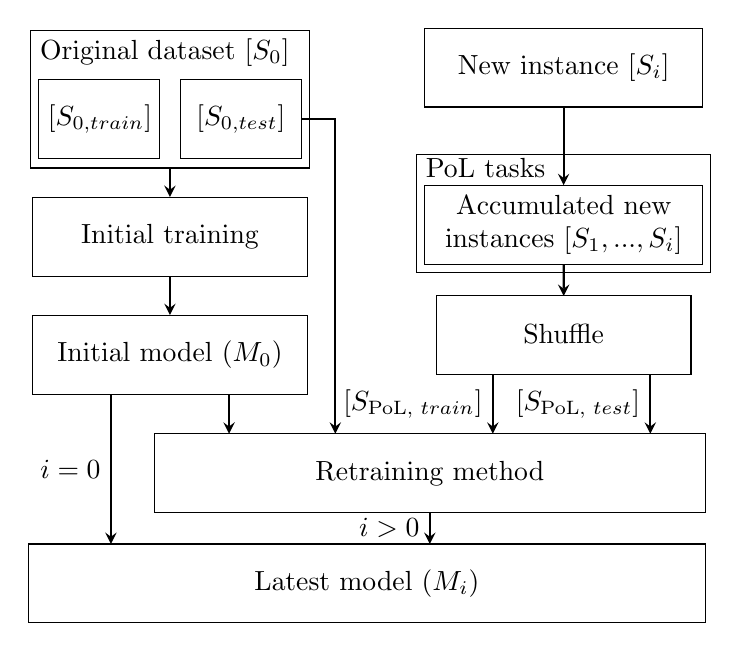
\begin{tikzpicture}[node distance=3.5cm]
   
    \node (original_dataset) [process, minimum width=3.5cm, minimum height=1.75cm, text width=3.3cm, text height=0cm, text depth = 1 cm, yshift=0cm, xshift=0cm, align=left] {Original dataset [$S_0$]};
    
    \node (original_dataset_train) [process, minimum width=1.25cm, text width=1.3cm, yshift=-0.25cm, xshift=-0.9cm] {[$S_{0,train}$]};
    
    \node (original_dataset_test) [process,  minimum width=1.25cm, text width=1.3cm, yshift=-0.25cm, xshift=0.9cm] {[$S_{0,test}$]};
    
    \node (initial_training) [process,  below of=original_dataset , yshift=1.75cm, xshift=0cm] {Initial training};
    
    \node (initial_model) [process,  below of=initial_training , yshift=2cm, xshift=0cm] {Initial model $(M_0)$};
    
    \node (retraining_method) [process, minimum width=7cm,  below of=initial_model , yshift=2cm, xshift=3.3cm] {Retraining method};
    
    \node (latest_model) [process, minimum width=8.6cm,  below of=initial_model , yshift=0.6cm, xshift=2.5cm] {Latest model $(M_{i})$};
    
    \node (new_instance) [process,  right of=initial_training, text width=3.3cm, yshift=2.15cm, xshift=1.5cm] {New instance [$S_{i}$]};
    
    % \node (oversampling) [process,  below of=new_instance, text width=3.3cm , yshift=2cm, xshift=0cm] {Create a distribution (Oversampling)};
    
    \node (PoL_tasks) [process, minimum width=3.5cm, minimum height=1.5cm, text width=3.5cm, text height=0cm, text depth = 0.9 cm, yshift=-1.45cm, xshift=5cm, align=left] {PoL tasks};
    
    \node (new_instances_storage) [process,  below of=new_instance, text width=3.3cm , yshift=1.5cm, xshift=0cm] {Accumulated new instances $[S_1,...,S_{i}]$};
    
    \node (shuffle) [process, minimum width=3cm, minimum height=1cm, text width=3cm, text height=0.2cm, text depth = 0cm, yshift=-3.0cm, xshift=5cm] {Shuffle};
    
      \draw[arrow] (4.1,-3.5) -- node[anchor=east] {$[S_{\text{PoL, }train}]$} (4.1,-4.25);
      
     \draw[arrow] (6.1, -3.5) -- node[anchor=east, yshift=0cm] {$[S_{\text{PoL, }test}]$} (6.1,-4.25);
    
    \draw [arrow] (original_dataset) -- (initial_training);
    
    \draw [arrow] (initial_training) -- (initial_model);
    
    \draw[arrow] (-0.75,-3.75) -- node[anchor=east] {$i=0$} (-0.75,-5.65);
    
    \draw[arrow] (0.75,-3.75) -- (0.75,-4.25);
    
    \draw[arrow] (3.3,-5.25) -- node[anchor=east] {$i>0$} (3.3,-5.65);
    
    % \draw [arrow] (original_dataset_test) -| node[anchor=south] {$S_{0,test}$} (2.5,-4.25);
    
    \draw [arrow] (original_dataset_test) -| (2.1,-4.25);
    
    \draw [arrow] (new_instance) -- (new_instances_storage);
    
    % \draw [arrow] (oversampling) -- (new_instances_storage);
    
    \draw [arrow] (new_instances_storage) -- (5,-2.5);

    \end{tikzpicture}
\caption{Retraining Pipeline}
\label{fig:retraining_pipeline2}
\end{figure}

\begin{figure}[h!]
    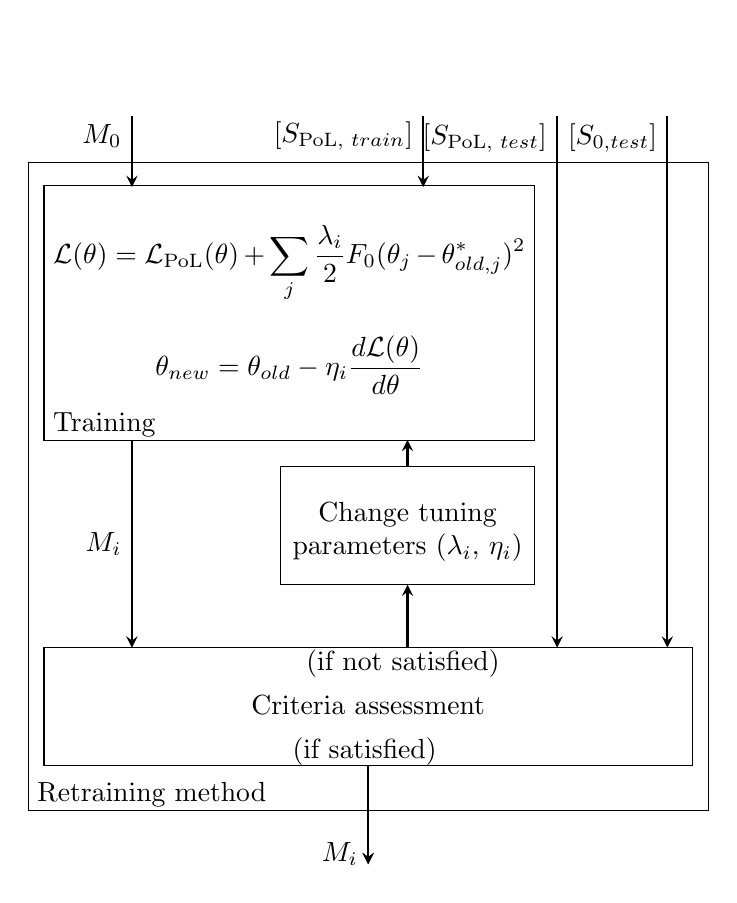
\begin{tikzpicture}[node distance=3.5cm]
   
    % \node (retraining_method) [process, minimum width=7cm, minimum height=10cm, text width=7cm, text height=10cm, text depth = 0 cm, yshift=0cm, xshift=0cm, align=left] {Retraining method};
    % \node (retraining_method) [process, fill=none, minimum width=4cm, minimum height=5cm, text width=8.4cm, text height=9cm, text depth = 0cm, yshift=-2.4cm, xshift=0cm, align=left] {Retraining method};
    
    \node (training_word) [process, draw=white, minimum width=4cm, minimum height=2cm, text width=8cm, text height=5cm, text depth = 0 cm, yshift=0cm, xshift=0cm, align=left] {Training};
    
    \node (training) [process, fill=none, minimum width=4cm, minimum height=2cm, text width=6cm, text height=0cm, text depth = 3cm, yshift=-1cm, xshift=-1cm, align=left] {\[\mathcal{L}(\theta) = \mathcal{L}_{\text{PoL}}(\theta) + \sum_{j}^{}\dfrac{\lambda_i}{2} F_0(\theta_j - \theta^{*}_{old,j})^2\]\\ \[\theta_{new} = \theta_{old} - \eta_{i} \dfrac{d\mathcal{L}(\theta)}{d\theta}\]};
    
    % \node (shuffle) [process, minimum width=3cm, minimum height=1cm, text width=3cm, text height=0.2cm, text depth = 0cm, yshift=2cm, xshift=2cm] {Shuffle};
    
    \node (change_parameters) [process, minimum width=3cm, minimum height=1.5cm, text width=3cm, text height=0cm, text depth = 0.1cm, yshift=-3.7cm, xshift=0.5cm] {Change tuning parameters ($\lambda_i$, $\eta_i$)};
    
    \node (criteria_assessment) [process, minimum width=8cm, minimum height=1.5cm, text width=8cm, text height=0.2cm, text depth = 0 cm, yshift=-6cm, xshift=0cm] {Criteria assessment};
    
    \draw[arrow] (-3,1.5) -- node[anchor=east,yshift=0.2cm] {$M_0$} (-3,0.6);
    
    \draw[arrow] (-3,-2.61) -- node[anchor=east] {$M_i$} (-3,-5.25);
    
    \draw[arrow] (0.5,-5.25) -- node[anchor=east,xshift=1.3cm,yshift =-0.6cm] {(if not satisfied)} (0.5,-4.45);
    \draw[arrow] (0.5,-2.95) -- node[anchor=east] {} (0.5,-2.61);
    
    % \draw[arrow] (2,3.5) -- node[anchor=east] {$[S_1,...,S_{i}]$} (2,2.5);
    
    % \draw[arrow] (0.9,1.5) -- node[anchor=east] {$[S_{(1,...,i),train}]$} (0.9,0.6);
    %  \draw[arrow] (3.1,1.5) -- node[anchor=east, yshift=2.92cm] {$[S_{(1,...,i),test}]$} (3.1,-5.25);
    
      \draw[arrow] (0.7,1.5) -- node[anchor=east, yshift=0.2cm] {$[S_{\text{PoL, }train}]$} (0.7,0.6);
      
     \draw[arrow] (2.4,1.5) -- node[anchor=east, yshift=3.1cm] {$[S_{\text{PoL, }test}]$} (2.4,-5.25);
    
     \draw[arrow] (3.8,1.5) -- node[anchor=east, yshift=3.1cm] {$[S_{0,test}]$} (3.8,-5.25);
     
     \draw[arrow] (0,-6.75) -- node[anchor=east,yshift =-0.5cm] {$M_i$} (0,-8);
     \draw[arrow] (0,-6.75) -- node[anchor=east,xshift=1cm,yshift =0.8cm] {(if satisfied)} (0,-8);
    
    
    % \node (training) [process, fill=none, minimum width=4cm, minimum height=5cm, text width=6cm, text height=0cm, text depth = 2cm, yshift=0cm, xshift=0cm, align=left] {\[\mathcal{L}(\theta) = \mathcal{L}_{new}(\theta) + \sum_{j}^{}\dfrac{\lambda_i}{2} F_0(\theta_j - \theta^{*}_{old,j})^2\]\\ \[\theta_{new} = \theta_{old} - lr_{i} \dfrac{d\mathcal{L}(\theta)}{d\theta}\]};
    
    % \node (assessment_criteria) [process, minimum width=1.5cm, minimum height=5cm, text width=1.7cm, text height=0cm, text depth = 0 cm, yshift=0cm, xshift=2.5cm] {Assessment criteria};
    % draw=black
    % \draw [arrow] (-4.5,0) --  node[anchor=south] {$[S_{0,test}]$} (-4,0);
    
    % \node (original_dataset_train) [process, minimum width=1.25cm, text width=1.3cm, yshift=-0.25cm, xshift=-0.9cm] {[$S_{0,train}$]};
    
    % \mathcal{L}(\theta) = \mathcal{L}_{B}(\theta) +  \sum_{i}^{} \frac{\lambda}{2} F^A_i (\theta_i - \theta^{*}_{A,i})^2
    
    % \draw [arrow] (initial_training) -- (initial_model);
    
    % \draw[arrow] (-0.75,-3.75) -- node[anchor=east] {$i=0$} (-0.75,-5.65);
    % \[ \sum_{n=1}^{\infty} 2^{-n} = 1 \]
    % \[\sum_{t=0}^{n}\dfrac{CF_t}{(1+r)^t}\]
    % $\mathcal{L}(\theta) = \mathcal{L}_{new}(\theta) + \sum{j}{}\lambda_i F_0(\theta_j - \theta^{*}_{old,j})^2$
    
    \node (retraining_method) [process, fill=none, minimum width=4cm, minimum height=5cm, text width=8.4cm, text height=8.0cm, text depth = 0cm, yshift=-3.2cm, xshift=0cm, align=left] {Retraining method};
    \end{tikzpicture}
\caption{Retraining Method}
\label{fig:retraining_method2}
\end{figure}

%
% In order for a DNN to improve its performance on a new task or an existent task, there need to be enough observations to allow the SGD to optimise for the new task i.e. complying with assumption~\assumptionSGDfirst. 
% %
% However, during operation there can be as little as one observation available to use for retraining.
% %
% One way to overcome this problem is through data augmentation techniques\footnote{Data augmentation are techniques used to enhance the size and quality of observations by adding slightly modified versions of the existing observations or by creating new observations inferred from existing observations~\cite{Shorten2019}.}, where small image rotations and shifts in the image frame are taken to create synthetic observations to populate the instance. 
%
The new instance $S_i$ gets appended to the accumulated new instances storage that represents the observations for the PoL tasks encountered during operation.
%
Note the $i^{th}$ counter used for the accumulated instances is not an indication of how many PoL tasks. 
%
They can all be instances of the same or different PoL tasks.
%
The observations for the PoL tasks then gets shuffled to become partly the retraining dataset $S_{\text{PoL, }train}$ and partly the test dataset $S_{\text{PoL, }test}$ for evaluating the retrained (latest) model, $M_i$, on the PoL tasks. 

At first, it can be thought why not learn PoL tasks sequentially and separately instead of sequentially and accumulated as we present in this paper? 
%
In other words why does the retraining dataset not contain observations only from the last new instance, and the previous new tasks get represented as separate EWC approximations using an additional Fisher matrix accompanied with an additional hyper-parameter ($\lambda$) to tune?
%
This has many challenges and may violate several of the assumptions established previously.
%
It cannot be guaranteed that the latest DNN model will be at a local minimum for all tasks represented by Fisher matrices, hence the validity of using a Fisher matrix to represent each of the previous PoL tasks might not always hold during operation.
%
Attempting to ensure all tasks represented by a Fisher are at a local minimum makes the tuning of the hyper-parameters i.e. the $\lambda$s extremely computationally expensive.
%
Additionally, The use of an EWC approximation or more specifically a Fisher matrix to represent a new task, can be said to violate assumption~\assumptionEWCsecond, because the approximation would not be for the overall distribution of the tasks in the operational environment.
%
Given the discussed limitations of learning PoL tasks sequentially and separately, we progressed with using sequentially and accumulated PoL tasks for retraining. 
%
Learning sequentially from accumulated observations would also result in retaining better performance of PoL tasks, as SGD is designed to optimise using random samples from the overall distribution as per assumption~\assumptionSGDfirst.

The training $S_{\text{PoL, }train}$ and testing $S_{\text{PoL, }test}$ datasets for the PoL tasks, the test dataset from the original tasks $S_{0,test}$, and the initial trained DNN model, $M_0$, are fed into the retraining method, which retrains to create the latest updated model ($M_i$). 
%
% A full representation of the retraining method is shown in
Figure~\ref{fig:retraining_method2} shows a more detailed diagram of the retraining method.
%
The starting model used in retraining at any $i^{th}$ retrain, is always the initial model $M_0$. This makes sure that assumption~\assumptionEWCfirst~relating to the DNN used in retraining is at a local minimum for the original tasks, hence ensuring the EWC approximation is valid to use.
%
In training, the mean squared error (see equation~\ref{eq:mean_square_loss}) is used to represent the loss function $\mathcal{L}_{\text{PoL}}(\theta)$ calculated over the observations from the PoL tasks training dataset (see Figure~\ref{fig:retraining_method2}), this can be replaced by other loss functions. On the other hand the original tasks are expressed using the EWC approximation. 
%
The $\theta_{old}$ and $\theta_{new}$ used in Figure~\ref{fig:retraining_method2} represent the previous and updated weights during training, respectively, similar to the explanation shown earlier in section~\ref{sec:gradient_decent}.

As was described earlier in section~\ref{sec:preliminaries}, there are two tuning parameters that can control the forgetting. 
%
The $\lambda$ represents the importance of the original tasks compared to the PoL tasks during retraining, the lower $\lambda$ is the less priority it is given during retraining, and if it is set to 0 then the original task will not be conserved using EWC. 
%
The other parameter is $\eta$, this constrains the rate at which the model being trained is allowed to deviate from its initial state. 
%
The lower $\eta$ is the more constrained the model is, if $\eta$ is 0 then the model will not change at all i.e. the PoL tasks will not be learnt.

Why are both of these tuning parameters needed? 
%
The SGD hyperparameter $\eta$ alone is not capable of optimising the retrained model alone on new tasks without resulting in significant forgetting. 
%
Conversely, relying only on tuning $\lambda$ to meet the criteria assessment can result in the retraining entering a state of instability where catastrophic forgetting will occur. 
%
This has been observed experimentally. However, the observation can be also explained by interpreting the mathematical calculations done in retraining. 
%
For example, if $\lambda$ is increased gradually whilst $\eta$ is fixed, at some point the value of $\lambda$ will result in the retraining steps taken by the SGD optimiser to be too large thus causing the model to diverge instead of converging to a local minimum. 
%
This happens due to the multiplication between $\lambda$ and $\eta$, shown in Equation~\ref{theta_new_substituted} that occurs when optimising the combined loss function $\mathcal{L}(\theta)$.
%
Equation~\ref{theta_new_substituted} is just a substitution of the equations shown in the training block in Figure~\ref{fig:retraining_method2}. 
%
Implicitly, $\lambda$ does have an effect on the learning rate due to this multiplication.
Hence an interplay of the two parameters is needed to allow for continuous stable training. 
\begin{equation}
   \theta_{new} = \theta_{old} - \eta_{i}\dfrac{\mathcal{L}_{\text{PoL}}(\theta)}{d\theta} - 
   \dfrac{\sum_{j}^{}\dfrac{\eta_i\lambda_i}{2} F_0(\theta_j - \theta^{*}_{old,j})^2}{d\theta}
   \label{theta_new_substituted}
\end{equation}

The criteria assessment block takes the retrained model $M_i$ and test it using the test datasets for the original tasks ($S_{0,test}$) and for the PoL tasks ($S_{\text{PoL, }test}$).
%
If the output matches the criteria set by the developers then the model $M_i$ is progressed to be used during operation, else the tuning parameters are tweaked to reach a retrained model that satisfies the criteria.
%
The criteria itself for learning during operation can be for example that the system should maximise its performance on PoL tasks whilst maintaining a performance of at least $90\%$ on the original tasks, to perhaps meet some regulatory conditions that a system was proved to have at deployment time. 


\section{Experimentation}\label{sec:experimentation}
The full code for the experimentation and results are available on: \url{https://github.com/Abanoub-G/EWC_PoL_Adaptation}.
% 
Experiments were run on a computer with an i7-10750H with 16GB RAM and an NVIDIA GeForce RTX 3060 graphics card, running Ubuntu 20.04.02 LTS.
\subsection{Datasets}
We use the popular 0-9 hand-written digits MNIST dataset~\cite{deng2012mnist}, divided into 10 classes, as the original dataset $S_0$ used in initial training.
% representing the original tasks used in initial training. 
%
This resembles the \textit{expected} operational environment of an
autonomous system, that was used at design time.
% The tasks learnt from the original dataset resembles the original tasks\textit{expected} in the operational environment of an autonomous system, that was used at design time.
%
The retraining and evaluation of our method is done using the n-MNIST~\cite{Basu2017} dataset, representing the \textit{actual} operational environment. 
% This is used to obtain new instances for retraining. 
%
The n-MNIST dataset has a similar pattern to the MNIST dataset but with three different types of noise applied to its tasks: Gaussian noise, blur, and reduced contrast with Gaussian noise. 
%
This makes it suitable to represent an operational environment of an autonomous system, where patterns of tasks encountered during operation are still similar to original tasks, but may have variations or noise that causes misclassifications.

\subsection{Implementation of retraining pipeline}
\subsubsection{Introduction of new instances}
To present a new instance that a DNN classifier may encounter during operation, an observation is selected randomly from the n-MNIST dataset.
%
Since the n-MNIST dataset is not a video feed dataset we use data augmentation techniques\footnote{Data augmentation are techniques used to enhance the size and quality of observations used in training by creating synthetic observations inferred from existing observations~\cite{Shorten2019}.} to create an instance from the randomly selected n-MNIST observation; where the synthetic observations here are small image rotations and shifts made to create the instance.
%
This was achieved using the image augmentation API provided by Keras\footnote{\url{https://www.tensorflow.org/api\_docs/python/tf/keras/preprocessing/\\image/ImageDataGenerator}}.  

The observations from each instance are split into 1000 training and 250 testing samples.
%
The test samples get evaluated on the latest retrained model ($M_i$).
%
If the test samples get misclassified i.e. accuracy is below the classification threshold, which is $50\%$, the instance counts as new and needs retraining. 
%
Otherwise, the process is repeated for another random observation from the n-MNIST dataset until a new instance is found.
%
The new instance gets added to the accumulated new instances storage whilst maintaining the 1000 to 250 split of training to testing samples. The training samples from the accumulated new instances are shuffled and then used to retrain the DNN classifier.
%
This process is repeated until the number of retraining episodes needed for the experiment is achieved.

\subsubsection{DNN Classifier}
% - What DNN was used, how it was constructed i.e. Pytorch etc.
A convolutional neural network (CNN) with three layers of convolutions and two fully connected layers was used to build the DNN classifier used in the experimentation. 
%
These specifications of the DNN were chosen based on its good performance on the MNIST dataset shown by other researchers\footnote{Example: \url{https://github.com/ContinualAI/colab/blob/master/notebooks}}.
%
An implementation of the EWC algorithm using Pytorch 1.8.1 with the DNN classifier used in the retraining pipeline was adopted and modified from the ContinualAI GitHub repository\footnote{\url{https://github.com/ContinualAI/colab}}.
%

\begin{figure*}[!t]
    \centering
    \begin{subfigure}{.3\textwidth}
        \includegraphics[width=1\textwidth]{../other/figures/98-115-4_v5.pdf}
        \caption{SGD \& EWC, Threshold: $98\%$}
        \label{98_box}
    \end{subfigure}
    \begin{subfigure}{.3\textwidth}
        \includegraphics[width=1\textwidth]{../other/figures/95-116-4_v3.pdf}
        \caption{SGD \& EWC, Threshold: $95\%$}
        \label{95_box}
    \end{subfigure}
    \begin{subfigure}{.3\textwidth}
        \includegraphics[width=1\textwidth]{../other/figures/90-117-4_v3.pdf}
        \caption{SGD \& EWC, Threshold: $90\%$}
        \label{90_box}
    \end{subfigure}
    
     \begin{subfigure}{.3\textwidth}
        \includegraphics[width=1\textwidth]{../other/figures/98-122-4_v1.pdf}
        \caption{SGD only, Threshold: $98\%$}
        \label{98_box_SGD}
    \end{subfigure}
    \begin{subfigure}{.3\textwidth}
        \includegraphics[width=1\textwidth]{../other/figures/95-123-4_v1.pdf}
        \caption{SGD only, Threshold: $95\%$}
        \label{95_box_SGD}
    \end{subfigure}
    \begin{subfigure}{.3\textwidth}
        \includegraphics[width=1\textwidth]{../other/figures/90-124-4_v1.pdf}
        \caption{SGD only, Threshold: $90\%$}
        \label{90_box_SGD}
    \end{subfigure}
    \caption{Spread of retrained model $M_i$ accuracy change on original and PoL tasks during 10 retraining episodes. Shown for EWC + SGD (i.e. tuning $\lambda$ and $\eta$) and SGD only (i.e. $\lambda = 0$ and tuning $\eta$) for controlled forgetting thresholds CF$_{\text{threshold}}$ of $98\%$, $95\%$ and $90\%$. }
    \label{fig:box}
\end{figure*}

% Criteria assessment
\subsubsection{Assessment Criteria}
The assessment criteria used in evaluating the performance of the retraining is shown in Algorithm~\ref{alg:assessment_criteria}.
%
\begin{algorithm}
\caption{Assessment criteria}\label{alg:assessment_criteria}
\begin{algorithmic}
\State orig$_{\text{acc}} = [\text{~}]$

\For{$\text{class} \text{ in } \text{classes}$}

\State {$\text{task}_{\text{test}} = S_{0, test}. \text{class}$}

\State $\text{acc} = M_i(\text{task}_{\text{test}})$

\State $\text{diff} = \text{CF}_{\text{threshold}} - \text{acc}$

\If{diff $> 0$}

    \State orig$_{\text{acc}}$.append(diff)
    
\EndIf


\EndFor

\State score$_{\text{original}} = sum$(orig$_{\text{acc}}$)

\State score$_{\text{PoL}} = 100 - M_i(S_{\text{PoL, }test})$

\State RS $= \text{score}_{\text{original}} + \text{score}_{\text{PoL}}$

\end{algorithmic}
\end{algorithm}
%
The assessment criteria aims at outputting a \textit{retraining score (RS)}, the smaller this score is the more the criterion is satisfied. When RS becomes zero then the criterion is fully satisfied. 
%
The RS is the sum of the \textit{original tasks score} (score$_{\text{original}}$) and the \textit{PoL tasks score} (score$_\text{{PoL}}$).
%
The score$_{original}$ approaches zero as the accuracy of the retrained model on each of the original tasks becomes equal or more than the \textit{controlled forgetting threshold (CF$_{\text{threshold}}$)}. 
%
This is a threshold that is set to control how much accuracy on the original tasks the system is allowed sacrifice during retraining. 
%
The score$_{\text{original}}$ is calculated as follows. An empty array (orig$_{\text{acc}}$) to store the accuracy on the original tasks is initiated. 
There are ten original tasks, each original task relates to one of the ten classes in the DNN. 
%
We loop over the ten original tasks and extract the test samples for that task from the $S_{0, test}$ dataset, these test samples are referred to as task$_{\text{test}}$.
%
The model $M_i$ accuracy (acc) is calculated on task$_{\text{test}}$.
%
If the accuracy is below the CF$_{\text{threshold}}$, then it gets appended to orig$_{\text{acc}}$. 
%
The score$_{\text{original}}$ is then computed as the sum of the members in orig$_{\text{acc}}$.

The PoL tasks score (score$_{\text{PoL}}$) is calculated differently, where all of the samples from the PoL tasks test dataset $S_{\text{PoL}, test}$ are evaluated on the retrained model without breaking it to into several tasks. This is subtracted from 100 since we want to maximise performance on PoL task.
%
Out of experimenting, this method of scoring for PoL tasks was found to yield better optimisation results than breaking the scoring to the individual PoL tasks as was done for the original tasks. 
%
This is because the number of observations available for each task of the PoL tasks is not the same as for the original tasks. 

% Tuning
We use \textit{Hyperopt}, a hyperparameters tuning algorithm based on Bayesian optimisation~\cite{Mockus1975,Snoek2012,Feurer2019}, to identify appropriate values for the hyperparameters $\lambda_i$ and $\eta_i$ to maximise the criterion satisfaction.

% \footnote{There are other optimisation algorithms that can be investigated e.g. Hyperband~\cite{Li2018d}, BOHB~\cite{Falkner2018}), to see which maximises the efficiency of the retraining, however we focus mainly on the classification accuracy improvements and control between the PoL tasks and the original tasks gained when EWC is used compared to its absence.}~\cite{bergstra13}. 

\section{Results and discussion}
% \begin{figure*}[!t]
%     \centering
%     \begin{subfigure}{.48\textwidth}
%         \includegraphics[width=1\textwidth]{other/figures/90-117-2_instances_v2.pdf}
%         \caption{Added Instance}
%         \label{fig:inst}
%     \end{subfigure}
%     \begin{subfigure}{.48\textwidth}
%         \includegraphics[width=1\textwidth]{other/figures/90-117-2_accumilated_v2.pdf}
%         \caption{Accumulated Instances}
%         \label{fig:_accum}
%     \end{subfigure}
%     \caption{Shows the classification accuracy of the first model $M_0$ from initial training, before last retrained model $M_{i-1}$ and the latest retraining model $M_i$ on (a) the added new instance $S_i$ and (b) the accumulated instances $[S_1,...S_i]$. The data presented here is for retraining with controlled threshold of 90\% on original tasks.}
%     \label{fig:Inst_accum}
% \end{figure*}
\begin{figure*}[!t]
    \centering
        \includegraphics[width=1\textwidth]{../other/figures/90-117-3_v2.pdf}
    \caption{Matrix plot showing accuracy change during retraining episodes, for controlled forgetting threshold of $90\%$, on each of the original tasks and the possible PoL tasks from the n-MNIST dataset. The red dots shows the instances that were added and at which retraining episode they were added from the ten retraining episodes.}
    \label{Matrix_plot}
\end{figure*}
%
% Discussion points: 
% - Discussion on important findings
%
Whilst using the $S_{\text{PoL, }test}$ dataset for evaluation during operation is the correct approach for assessing the satisfaction of the retraining criterion, to study our research questions we need a larger pool of data to understand the performance generalisation from operational retraining.
%
Therefore, conversely to the assessment criteria which uses the test dataset $S_{\text{PoL, }test}$ obtained from the accumulated instances storage, we use the overall test dataset provided in the n-MNIST dataset to investigate our research questions.
% therefore, answering our two research questions. 
%
% We use the test dataset provided in the n-MNIST dataset to study how well forgetting is controlled and whether the retraining generalises, therefore, answering our two research questions.
%
% We first discuss the feasibility of a system self-assessing its performance gain on PoL tasks using the $S_{\text{PoL, }test}$ test dataset.
%
We base all of the results presented here on ten consecutive retraining episodes for ten new instances.

\subsection{EWC+SGD vs SGD alone}
Figure~\ref{fig:box} aims at answering \textbf{RQ1}, to show how the presence of EWC reduces forgetting and still allows the the classifier to adapt to PoL tasks.
%
There are ten original tasks for the ten digits 0-9 in the MNIST dataset. 
%
The test samples for each of those tasks is assessed on the latest retrained model $M_i$ and the initial model $M_0$ after every retrain. 
%
The two outputs of this evaluation are subtracted from each other giving the \textit{accuracy change}, i.e. gain or loss in performance compared to the initial model. 
%
The accuracy change is shown by y-axis in the Figure~\ref{fig:box} and the red dotted line refers to zero change in accuracy from the first model's $M_0$ accuracy on any given task. 
% 
The spread of accuracy change on the ten original tasks for all ten retraining episodes is grouped and shown by the box for original tasks in Figure~\ref{fig:box}.

Similarly, for the PoL tasks, after every retrain the relevant test samples from the n-MNIST for the PoL tasks are assessed on the latest retrained model $M_i$ and the initial model $M_0$ to calculate the accuracy change.
%
Note the n-MNIST has 30 tasks (10 classes $\times$ 3 noise types). 
%
Not all 30 tasks are PoL tasks. 
%
The relevant tasks from the n-MNIST for which we use test samples, after every retrain, depends on the instances that were used in retraining. 
%
For example, if the model is retrained on four instances that are extracted from two tasks from the n-MNIST dataset, then there would be only two PoL tasks, for which we need to test for accuracy change. 
%
Then assuming the fifth instance belongs to another third task from the n-MNIST then there would be three PoL tasks, for which we need to test for accuracy change.  
%
This way we collect the accuracy change for the PoL tasks grouped in the box plot in Figure ~\ref{fig:box}.

The six plots in Figure ~\ref{fig:box} show the accuracy change on original and PoL tasks, for three controlled forgetting thresholds CF$_{\text{threshold}}$: $98\%$,  $95\%$ and $90\%$.
%
The box denotes the interquartile range of accuracy change, non-outlier limits by the whiskers and a horizontal bar for the median. 
%
For all three thresholds used in experimentation, the EWC+SGD shows a much more controlled forgetting paradigm on the original tasks compared to SGD only. 
%
This is evident by the very low spread of accuracy change close to the red dotted lines for the EWC+SGD and the very sparse accuracy change below the red dotted line for the SGD only.
%
This shows that the SGD only approach results in significant model drift and even catastrophic forgetting of some tasks, even at very high controlled forgetting thresholds (see Figure~\ref{98_box_SGD}).
%
For both EWC+SGD and SGD only the PoL tasks seem to generally improve in accuracy. 
%
The SGD only achieves slightly higher performance but more sparsed on PoL tasks compared of EWC+SGD. 
%
This may have merits depending on applications but also indicates overfitting to PoL tasks which is actually the case since the forgetting is much more significant when using SGD only.   

% - Comparison of results on SGD+EWC with SGD only

% \subsection{Performance gain and generalisation for autonomous systems adaptation}
\subsection{Generalisation on PoL tasks}
% Figure~\ref{fig:Inst_accum} shows the before and after retraining accuracy on (a) the latest added new instance in the retraining episode and the (b)accumulated instances. The grey bar is the classification accuracy of the first model $M_0$. The white bar is the performance of the before last retrained model $M_{i-1}$ whilst the black bar is the accuracy of the latest retrained model $M_i$.  
% %
% Overall the retraining is causing the classification accuracy to increase on the individual instances and on the overall accumulated instances compared to the first model. 
% %
% Even though some instances do not pass the classification threshold like at retraining episode 6 in Figure~\ref{fig:inst}, which means they are still misclassified as instances but it still has a positive impact on the classifiers generalisation on the task, as can be seen in Figure~\ref{Matrix_plot}.

Figure~\ref{Matrix_plot}~ gives a more insightful look at the generalisation on the PoL tasks of the system. 
%
This matrix diagram shows a subplot for each of the ten  original tasks (learnt from MNIST) and the thirty potential PoL tasks (provided by n-MNIST) that may become part of the system's operational environment.  
% (RQ2): Does learning from a limited number of relevant observations generalises the classifier’s performance to the new tasks?
%
To investigate \textbf{RQ2}, a matrix plot displaying the accuracy of the initial model $M_0$ and the latest model $M_i$ on all of the tasks in the MNIST (row labelled ``\textbf{Original}'' ) and n-MNIST (rows labelled ``\textbf{Noise 1}'', ``\textbf{Noise 2}'', and ``\textbf{Noise 3}'' ) datasets through out the ten retraining episodes is shown in Figure~\ref{Matrix_plot}.  
%
All of the MNIST tasks are the original tasks and the n-MNIST tasks with red dots are the PoL tasks. 
A task from the n-MNIST tasks
% The classifier accuracy on a task from noise 0, 1 or 2
only becomes of a PoL task after an instance of it appears in the system's operational environment. 
%
% This indicates that the task has become part of the system's operational environment. 
%
The appearance of the instances is denoted by the red dot, showing at which retraining episode an instance from that task was used in retraining.

To assess on generalisation, as was discussed previously, a larger pool of test samples is needed than in the $S_{\text{PoL, }test}$.
%
Therefore, again the test samples are extracted for each task from the overall test samples availble from the MNIST and n-MNIST datasets.
%
% The evaluation plotted on these subplots is done using the test datasets provided by MNIST and n-MNISt for each of their tasks i.e. similar to the box plots shown earlier, the test datasets are not from the accumulated instances dataset that was used in retraining.
%
% This data usually is not available for a system encountering instances of new tasks during operation, but is used here to study how the system generalises on other observations coming from the same task. 

% Demonstrated by
Observing the solid black lines (accuracy of $M_i$) and the red dotted lines (accuracy of $M_0$) in Figure~\ref{Matrix_plot}, it is evident that after the classifier is retrained on a new instance the accuracy of the PoL task the instance comes from improves beyond the initial model's accuracy showing positive adaptation to the generalised PoL tasks.  
% classifiers capability on the same task using the first model $M_0$. 
% 
This is achieved at the expense of some forgetting of the original tasks, which is acceptable given that the model is drifting to fit its \textit{pattern of life}.    
%
Furthermore, there is drop in accuracy on other tasks from the n-MNIST dataset that have not become PoL tasks, this is not of concern as these other tasks fall out of the operational design domain of the system i.e. they are not part of the original tasks nor have been identified as PoL tasks.
% - Strength and limitations of the study

% It is challenging to assess the generalisation of the DNN classifier on new tasks just by evaluating its accuracy on the available observations, as was demonstrated by the earlier discussion on Figure~\ref{Matrix_plot}. 
%
% This may introduce limitations on the system's capability of monitoring and assessing its generalisation behaviour on new tasks from a few new instances. 
%
% However, monitoring the improvement on new instances classification can be an indicator of good or bad generalisation. For example improved accuracy can be a positive sign, but achieving really high accuracy on all of the new instances can be a sign of overfitting and thus poor generalisation.

\subsection{Retraining speed}
A limitation of the current retraining pipeline is that as more new instances appear the retraining process will become slower as there are more observations to optimise the model for in the accumulated new instances storage.
%
This limitation might be mitigated by decreasing or more generally adjusting the number of observations used in retraining from each new instance captured in the accumulated instance storage as the number of new instances increase.

Removal of instances from the accumulated storage of instances for PoL tasks that the system has not encountered in along period of time, thus is not part of the \textit{pattern of life} of the system anymore.
%
% may be limited by decreasing oversamples of the instances in the accumulated new instances storage used in retraining as the number of new instances increase. 
%
% Removal of instances completely from the storage that does not fall into the PoL of the system any more can be another approach for tackling this limitation. 
%
A way of achieving that can be by keeping track of how often the system encounters similar instances (perhaps by using dissimilarity measures~\cite{Hond2020} to detect them), and decide whether it is beneficial to remove or keep certain instances based on some criteria put by developers or regulators. 

If the system is encountering a large number of new instances all falling in its PoL then that may invite for developers to investigate the observations used in initial training, as the expected and actual operational environments are very different. 

\subsection{A Note on transfer learning}
Learning from a few observations is
% as little as one instance is
generally challenging and does not abide with current machine learning paradigms, which relies on the availability of abundant observations to learn new tasks. 
%
Using data augmentation techniques, as done in the experimentation, certainly improves learning of the new tasks and its generalisation. 
%
However a major contribution to the success of our method is caused by transfer learning obtained from original tasks. 
%
This poses a limitation in the use of the proposed approach from learning tasks following a completely different pattern, e.g Permuted-MNIST~\cite{Goodfellow2014} or Fashion-MNIST~\cite{Xiao2017}, which extends beyond the scope of our work.
% which aims at increasing the reliability of autonomous systems on tasks in its operational environment that have some variations such as a novel type of noise as opposed to a completely novel pattern.


\section{Conclusions}\label{sec:conclusions}
In this paper, we have demonstrated that using  EWC allows for more controlled learning of new tasks from new instances whilst controlling the limit allowed for forgetting of original tasks.
This was followed by studying the gains in accuracy and generalisation of retrained DNN classifiers on new tasks using the MNIST and the n-MNIST datasets to represent expected and actual operational environments, respectively. 
%
Thus gain an understanding of using this method for pattern of life adaption of autonomous systems. 
%
The results show that there are clear signs of generalisation on pattern of life tasks from retraining on limited observations of new instances derived from these pattern of life tasks.
%
\subsection{Future works}\label{sec:future_works}
Posing questions for future works to allow for the adoption of this retraining pipeline in real-time autonomous systems include:
\begin{itemize}
    \item Developing runtime monitors to help an autonomous system evaluate its performance on PoL tasks after retrains inferred from the classifiers accuracy improvement on encountered new instances.
%
   \item Investigate methods for maintaining the retraining speed of the DNN classifier as the new instances storage increases to still allow for efficient retraining.
   
    % \item Investigate the possibility of updating the fisher matrix with out introducing new lambdas? Exploration of the EWC approximations to yeild better learning results for continual learning like \cite{Chen2019b}. 
\end{itemize}

\section*{Acknowledgments}
This research is part of an iCASE PhD funded by EPSRC and Thales UK. Special thanks to 
% Darryl Hond from Thales UK and 
Edwin Simpson from University of Bristol for helping with reviewing the paper.

% ***************************************************
%  Bib
% ***************************************************
\printbibliography

% ***************************************************
%  Bio
% ***************************************************

\begin{IEEEbiography}[{\includegraphics[width=1in,height=1.25in,clip,keepaspectratio]{../other/mugs/abanoub}}]{Abanoub Ghobrial}
received the MEng degree in mechanical engineering from the University of Bristol, Bristol,  U.K., in 2018. He is currently pursuing the Ph.D. degree in computer science at the University of Bristol and is a part-time Research Associate with the Trustworthy Systems Lab, Bristol,  U.K. From 2018 to 2020, he was a full-time Research Associate with the Trustworthy Systems Lab. His current research interests are techniques to allow self-managing of autonomous safety-critical systems via continual learning during operation; and the development of simulation-based verification techniques for autonomous systems.
\end{IEEEbiography}


\begin{IEEEbiography}[{\includegraphics[width=1in,height=1.25in,clip,keepaspectratio]{../other/mugs/kie}}]{{Kerstin Eder}} 
is Professor of Computer Science and heads the Trustworthy Systems Laboratory at the University of Bristol, UK. She also leads the Verification and Validation for Safety in Robots research theme at the  Bristol Robotics Laboratory. She has gained extensive experience of verifying complex microelectronic designs while working with leading semiconductor design and Electronic Design Automation companies worldwide. Her research is focused on specification, verification and analysis techniques to verify or explore a system's behaviour in terms of functional correctness, safety, security, performance and energy efficiency. Prof.\ Eder's most recent contributions include agent-based testing, how to use assertions and theorem proving to verify control system designs, energy modeling and static resource analysis techniques to predict energy consumption of software. She holds a PhD in Computational Logic and an MSc in Artificial Intelligence from the University of Bristol, UK, as well as an MEng in Informatics (Dipl.\,Inf.) from the Technical University Dresden, Germany. In 2007 she was awarded an ``Excellence in Engineering'' prize from the Royal Academy of Engineering, UK.

\end{IEEEbiography}


% ***************************************************
%  Appendix
% ***************************************************

\end{document}
